% coding:utf-8

%FOSASTOC, a LaTeX-Code for a electrical summary of stochastic
%Copyright (C) 2013, Daniel Winz, Ervin Mazlagic

%This program is free software; you can redistribute it and/or
%modify it under the terms of the GNU General Public License
%as published by the Free Software Foundation; either version 2
%of the License, or (at your option) any later version.

%This program is distributed in the hope that it will be useful,
%but WITHOUT ANY WARRANTY; without even the implied warranty of
%MERCHANTABILITY or FITNESS FOR A PARTICULAR PURPOSE.  See the
%GNU General Public License for more details.
%----------------------------------------

\section{Grundbegriffe}

\subsection{R-Tipps}
\subsubsection{Zahlenfolgen definieren}
Vektor für eine lineare Zahlenfolge definieren mit Intervall = 1
\begin{Schunk}
\begin{Sinput}
> x <- 1:10
> x
\end{Sinput}
\begin{Soutput}
 [1]  1  2  3  4  5  6  7  8  9 10
\end{Soutput}
\end{Schunk}
Vektor für eine Zahlenfolge mit beliebigem Intervall (z.B. 3)
\begin{Schunk}
\begin{Sinput}
> x <- seq(1,20,3)
> x
\end{Sinput}
\begin{Soutput}
[1]  1  4  7 10 13 16 19
\end{Soutput}
\end{Schunk}
Eine spezielle Zahlenfolge kann auch manuell definiert werden
\begin{Schunk}
\begin{Sinput}
> x <- c(3,2,5,8,9,10,55,1,12)
> x
\end{Sinput}
\begin{Soutput}
[1]  3  2  5  8  9 10 55  1 12
\end{Soutput}
\end{Schunk}

\subsection{Artihmetisches Mittel}
Das arithmetische Mittel beschreibt den Mittelwert der Summe aller Elemente.

\[ \bar{x} = \frac{1}{n} \sum\limits_{i=1}^{n} x_i \]

\subsubsection{Artihmetisches Mittel mit R berechnen}
Mit R kann das arithmetische Mittel mit der Funktion \verb!mean()! 
ermittelt werden
\begin{Schunk}
\begin{Sinput}
> x <- c(2,5,1,7,8,9)
> mean(x)
\end{Sinput}
\begin{Soutput}
[1] 5.333333
\end{Soutput}
\end{Schunk}

\subsection{Standardabweichung}
Die Standardabweichung beschreibt wie gross die mittlere Abweichung der
Beobachtungen vom arithmetischen Mittel derselben Beobachtungen ist.
\[ s_x = \sqrt{ \frac{1}{n-1} \sum\limits_{i=1}^{n} (x_i - \bar{x})^2 } \]
Bsp.: Wir nehmen eine zufällige Zahlenfolge innerhalb $(1,10)$ und
rechnen das arithmetische Mittel als auch die Standardabweichung (\verb!sd()!).
\begin{Schunk}
\begin{Sinput}
> x <- round(x=runif(n=10, min=1, max=10), digits=0)
> x
\end{Sinput}
\begin{Soutput}
 [1] 2 6 8 7 9 8 5 2 4 7
\end{Soutput}
\begin{Sinput}
> mean(x)
\end{Sinput}
\begin{Soutput}
[1] 5.8
\end{Soutput}
\begin{Sinput}
> sd(x)
\end{Sinput}
\begin{Soutput}
[1] 2.485514
\end{Soutput}
\end{Schunk}

\subsection{Quantile}
Quantile beschreiben folgenden Zusammenhang: Hat man z.B. 20 Messungen gemacht
und sortiert diese, dann beschreibt ein x\%-iges Qantil eine Punkt oder Grenze
in der Messreihe, wo x\% der Werte darunter liegen.

\[ \alpha: \text{ Prozentwert} \quad \alpha \in [0,1] \]
\[ x_1 - x_n \text{ sortiert nach grösse}  \]
\[ \alpha \cdot n \]
\[ \text{hier müssen 2 Fälle unterschieden werden: ganze Zahlen und gebrochene} \]
\[ \text{ganze Zahlen:} \quad \frac{1}{2} 
\cdot (x_{\alpha \cdot n} + x_{\alpha \cdot (n+1)}) \]
\[ \begin{array}{@{}@{}ll}
	\text{gebrochene Zahlen:} & k=\alpha \cdot n + \frac{1}{2} \\
	                          & k \text{ runden} \\
				  & \Rightarrow x_{(k)}
\end{array}\]

\begin{Schunk}
\begin{Sinput}
> x<-round(x=runif(n=20, min=1, max=20), digits=0)
> x<-sort(x)
> x
\end{Sinput}
\begin{Soutput}
 [1]  2  2  2  2  2  3  4  7  7  8  8  9  9  9 13 14 15 15 18 19
\end{Soutput}
\begin{Sinput}
> quantile(x, prob=0.2)
\end{Sinput}
\begin{Soutput}
20% 
  2 
\end{Soutput}
\begin{Sinput}
> quantile(x, prob=0.2, type=1)
\end{Sinput}
\begin{Soutput}
20% 
  2 
\end{Soutput}
\begin{Sinput}
> quantile(x, prob=0.2, type=2)
\end{Sinput}
\begin{Soutput}
20% 
  2 
\end{Soutput}
\end{Schunk}
Im obigen Beispiel wird mit R das 20\%-Quantil bestimmt. Hier ist aber 
Vorsicht geboten, denn R hat 9 verschiedene \verb!type! für die Funktion
\verb!quantile()! (default-Wert ist 7). Für uns aus dem 
Stochastik-Modul ist der \verb!type=2! 
der einzig richtige Wert!

\subsection{Median}
Der Median ist ein Spezialfall der Quantile, nämlich ist dies jenes Quantil,
welches die 50\%-Marke beschreibt.

Bsp.: Wir haben 5 Personen, und messen deren Höhe. Danach sortieren wir die
Ergebnisse. Der Median ist nun jene Person in der Mitte (unabhängig von seiner
genauen Höhe!). Interssant oder eben speziell am Median ist,
dass es immer die selbe Person bleibt auch wenn die kleineren und grösseren
noch grösser und noch kleiner werden. Dies bedeutet, dass der Median 
unempfindlich gegenüber sog. Ausreissern ist (denke an Durchschnittsvermögen
in einem Land mit vielen Armen und wenigen aber extrem Reichen).
\begin{Schunk}
\begin{Sinput}
> x <- c(1.6, 1.7, 1.75, 1.87, 1.94)
> median(x)
\end{Sinput}
\begin{Soutput}
[1] 1.75
\end{Soutput}
\begin{Sinput}
> x <- c(1.2, 1.4, 1.75, 1.99, 2.14)
> median(x)
\end{Sinput}
\begin{Soutput}
[1] 1.75
\end{Soutput}
\end{Schunk}

\subsection{Varianz}
Die Varianz beschreibt die quadratische Abweichung von Daten von ihrem 
arithmetischen Mittelwert. Sie ist das Quadrat der Standardabweichung. 
\[ {s_x}^2 = \frac{1}{n-1} \sum\limits_{i=1}^{n} (x_i - \bar{x})^2 \]
\begin{Schunk}
\begin{Sinput}
> x=runif(n=10)
> y=runif(n=10)
> var(x)
\end{Sinput}
\begin{Soutput}
[1] 0.09006661
\end{Soutput}
\end{Schunk}

\subsection{Kovarianz}
Die Kovarianz beschreibt, wie stark die Abweichungen von zwei Vektoren von 
ihren jeweiligen arithmetischen Mittelwerten korrelieren. Die Kovarianz 
eines Vektors mit sich selbst entspricht der Varianz des Vektors. 
\[ s_{xy} 
= \frac{1}{n-1} \sum\limits_{i=1}^{n} (x_i - \bar{x}) (y_i - \bar{y}) \]
\begin{Schunk}
\begin{Sinput}
> cov(x,y)
\end{Sinput}
\begin{Soutput}
[1] -0.04171591
\end{Soutput}
\end{Schunk}

\subsection{Korrelationskoeffizient}
Der Korrelationskoeffizient beschreibt die Linearität von zwei Vektoren 
zueinander. Der Wertebereich des Korrelationskoeffizienten ist $[-1, 1]$. 
\[ r = \frac{s_{xy}}{s_x \cdot s_y} 
= \frac{\sum\limits_{i=1}^{n} (x_i - \bar{x}) (y_i - \bar{y})}
{\sqrt{\sum\limits_{i=1}^{n} (x_i - \bar{x})^2  \cdot 
\sum\limits_{i=1}^{n} (y_i - \bar{y})^2 }} \]
\begin{Schunk}
\begin{Sinput}
> cor(x,y)
\end{Sinput}
\begin{Soutput}
[1] -0.4500696
\end{Soutput}
\end{Schunk}

\section{Kombinatorik}
$A$ und $B$ sind stochastisch unabhängig. 
\[ P(A) \geq 0 \]
\[ P(\Omega) = 1 \qquad \text{(Grundraum)} \]
\[ P(A \cup B) = P(A) + P(B) \qquad \text{Falls } A \cap B = 0 
\qquad \text{($A$ und $B$ schliessen sich aus)} \]
\[ P(A \cup B) = P(A) + P(B) - P(A \cap B) \qquad \text{(Additionsgesetz)} \]
\[ P(A \cap B) = P(A) \cdot P(B) \]
\[ P(A \cap B \cap C) = P(A) \cdot P(B) \cdot P(C) \]
\[ P(A') = 1 - P(A) \]

\subsection{Diskrete Wahrscheinlichkeit}
\[ P(E) = \frac{\text{\# positive Elementarereignisse}}
{\text{\# mögliche Elementarereignisse}} \]

\newpage
\section{Bedingte Wahrscheinlichkeit}
Bei bedingten Wahrscheinlichkeiten gilt das sog. Beyes'sche Theorem.
\[ \boxed{ P_B(A) = P(A|B) = \frac{P(A \cap B)}{P(B)} = \frac{P(B|A)\cdot P(A)}{P(B)} } \]
\[ \boxed{P(B) = P(B|A) \cdot P(A) + P(B|A') \cdot P(A')} \]
\[ \boxed{P(B) = P(B \cap A) \cdot P(A) + P(B|A') \cdot P(A')} \]

\begin{figure}[h!]
        \centering
        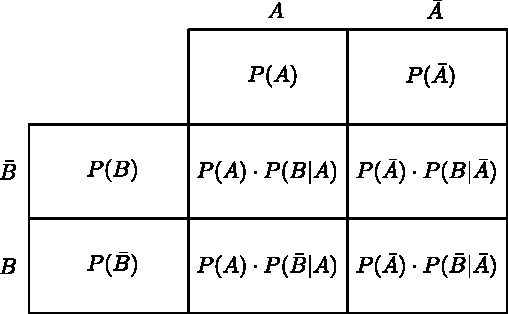
\includegraphics[scale=\graphscale]{bedingte-wahrscheinlichkeit.pdf}
        \caption{Übersicht zur Berechnung der bedingten Wahrscheinlichkeiten}
\end{figure}

\begin{figure}[h!]
        \centering
        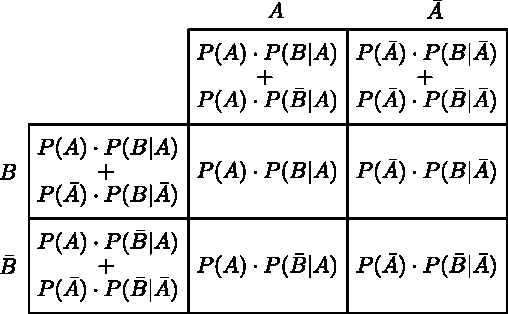
\includegraphics[scale=\graphscale]{bedingte-wahrscheinlichkeit-detail.pdf}
        \caption{Übersicht mit berechneten Wahrscheinlichkeiten der Ereignisse}
\end{figure}

\begin{figure}[h!]
        \centering
        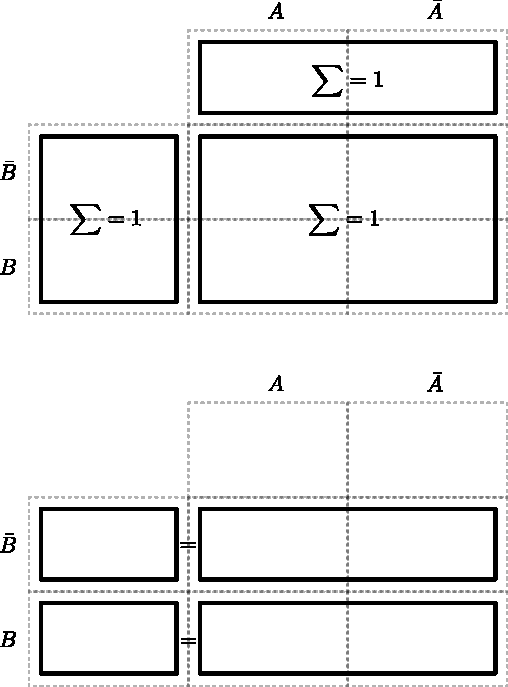
\includegraphics[scale=\graphscalesmall]{bedingte-wahrscheinlichkeit-tipps.pdf}
        \caption{Tipps zu Zusammenhängen bei bedingten Wahrscheinlichkeiten}
\end{figure}

\newpage
\section{Lineare Transformation}
Wird eine Zufallsvariable linear transformiert, müssen auch der Erwartungswert 
$E(X)$ und die Varianz $Var(X)$ transformiert werden. 
\[ Y = a \cdot X + b \]
\[ \rightarrow E(Y) = a \cdot E(X) + b \]
\[ \rightarrow Var(Y) = a^2 \cdot Var(X) \]

\section{Diskrete Verteilungen}

\subsection{Hypergeometrische Verteilung}
Die Hypergeometrische Verteilung beschreibt die Wahrscheinlichkeit beim 
Ziehen ohne zurücklegen. Im folgenden Beispiel mit farbigen Kugeln. 
\[ X \sim Hyp(n, r, s) \]
\begin{tabular}{@{}ll}
  $n$: & Anzahl Ziehungen \\
  $r$: & Anzahl rote Kugeln in der Urne (positive Ergebnisse) \\
  $s$: & Anzahl schwarze Kugeln in der Urne (negative Ergebnisse) \\
  $N$: & Anzahl Kugeln in der Urne ($N = r + s$)
\end{tabular}
\[ P(X=k) 
= \frac{\left( \begin{array}{c}r\\k\end{array} \right) \cdot 
\left( \begin{array}{c}s\\n-k\end{array} \right)}
{\left( \begin{array}{c}r+s\\n\end{array} \right)} 
= \frac{\left( \begin{array}{c}r\\k\end{array} \right) \cdot 
\left( \begin{array}{c}N-r\\n-k\end{array} \right)}
{\left( \begin{array}{c}N\\n\end{array} \right)} \]
\begin{Schunk}
\begin{Sinput}
> k=6;
> n=6;
> r=6;
> s=36;
> dhyper(x=k,m=r,n=s,k=n)
\end{Sinput}
\begin{Soutput}
[1] 1.906292e-07
\end{Soutput}
\end{Schunk}

\subsubsection{Erwartungswert}
\[ E(X) = n \cdot \frac{r}{N} \]
\subsubsection{Varianz}
\[ Var(X) = n \cdot \frac{r}{N} \cdot \left(1 - \frac{r}{N}\right) 
\cdot \frac{N - n}{N - 1} \]

\subsubsection{Kumulative Verteilungsfunktion}
\begin{Schunk}
\begin{Sinput}
> q=1;
> phyper(q=q,m=r,n=s,k=n)
\end{Sinput}
\begin{Soutput}
[1] 0.8025001
\end{Soutput}
\end{Schunk}

\subsection{Binomialverteilung}
Die Binomialverteilung kann bei Ereignissen eingesetzt werden, die zwei 
mögliche Ergebnisse zeigen können. Sie ist ein Grenzfall der 
Hypergeometrischen Verteilung. 
\footnote{Beispiele für Ereignisse mit zwei möglichen Ergebnissen: 
  \begin{itemize} 
    \item Münzwurf $\Rightarrow$ Kopf $\leftrightarrow$ Zahl
    \item Würfeln $\Rightarrow$ Sechser $\leftrightarrow$ kein Sechser
  \end{itemize}}
Die Wahrscheinlichkeit ist dann wie folgt gegeben: 
\[ P(X=x) = 
\left( \begin{array}{c}n\\x\end{array} \right) \cdot p^x \cdot (1-p)^{n-x} 
= \frac{n!}{x! (n-x)!} \cdot p^x \cdot (1-p)^{n-x} \]
\[ X \sim Bin(n,p) \]
\begin{tabular}{@{}ll}
  $n$: & Anzahl Versuche \\
  $x$: & Anzahl Versuche mit positivem Ergebnis \\
  $p$: & Wahrscheinlichkeit für ein positives Ergebnis bei jedem einzelnen Versuch
\end{tabular} 
\begin{Schunk}
\begin{Sinput}
> n=5;
> x=3;
> p=0.2;
> dbinom(x=x,size=n,prob=p)
\end{Sinput}
\begin{Soutput}
[1] 0.0512
\end{Soutput}
\end{Schunk}

\subsubsection{Erwartungswert}
\[ E(X) = n \cdot p \]

\subsubsection{Varianz}
\[ Var(X) = n \cdot p \cdot (1 - p) \]

\subsubsection{Kumulative Verteilungsfunktion}
\begin{Schunk}
\begin{Sinput}
> q=3;
> pbinom(q=q,size=n,prob=p)
\end{Sinput}
\begin{Soutput}
[1] 0.99328
\end{Soutput}
\end{Schunk}

\subsection{Poissonverteilung}
Die Poissonverteilung wird bei Ereignissen verwendet, deren maximale Anzahl 
nicht begrenzt ist. Sie ist ein Grenzfall der Binomialverteilung. 
\[ P(X=x) = \exp(-\lambda) \cdot \frac{\lambda^x}{x!} \]
\[ X \sim Pois(\lambda) \]
\begin{tabular}{@{}ll}
  $x$: & Anzahl Versuche mit positivem Ergebnis \\
  $\lambda$: & Erwartungswert
\end{tabular} 
\begin{Schunk}
\begin{Sinput}
> lambda=2;
> x=3;
> dpois(x=x,lambda=lambda)
\end{Sinput}
\begin{Soutput}
[1] 0.180447
\end{Soutput}
\end{Schunk}

\subsubsection{Erwartungswert}
\[ E(X) = \lambda \]

\subsubsection{Varianz}
\[ Var(X) = \lambda^2 + \lambda \]

\subsubsection{Kumulative Verteilungsfunktion}
\begin{Schunk}
\begin{Sinput}
> q=3;
> ppois(q=q,lambda=lambda)
\end{Sinput}
\begin{Soutput}
[1] 0.8571235
\end{Soutput}
\end{Schunk}

\subsection{Übersicht Berechnung diskreter Verteilungen mit R}
\begin{tabular}{@{}lllll}
  \rowcolor{lgray}Verteilung &
    genau & 
    höchstens & 
    mindestens &
    Zufall  \\
  Hyper &
    \verb!dhyper(x=A,...)! &
    \verb!phyper(q=A,...)! &
    \verb!1-phyper(q=A-1,...)! &
    \verb!rhyper(n=...)! \\
  Binom &
    \verb!dbinom(x=A,...)! &
    \verb!pbinom(q=A,...)! &
    \verb!1-pbinom(q=A-1,...)! &
    \verb!rbinom(n=...)! \\
  Poisson &
    \verb!dpois(x=A,...)! &
    \verb!ppois(q=A,...)! &
    \verb!1-ppois(q=A-1,...)! &
    \verb!rpois(n=...)!
\end{tabular}

\section{Stetige Verteilungen}

\subsection{Dichtefunktion}
Die Dichtefunktion ist definiert als Ableitung der kummulativen 
Verteilungsfunktion.
\[ \int f(x) := F(x) \qquad \Leftrightarrow \qquad
   f(x) = \frac{d}{d x} F(x)  \]

   \begin{figure}[h!]
           \centering
           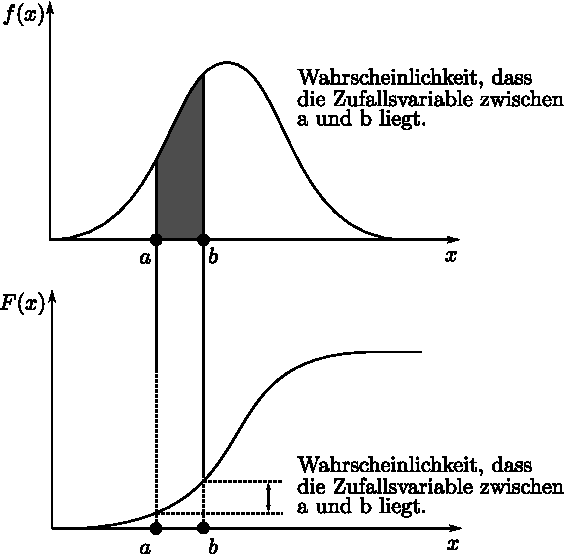
\includegraphics[scale=\graphscale]{dichtefunktion.pdf}
           \caption{Dichtefunktion $f(x)$ und kummulative Verteilungsfunktion $F(x)$.}
   \end{figure}

\noindent
Dies impliziert, dass auch die folgenden Gesetzte gelten:
\begin{itemize}
	\item Die Dichte zu einem Punkt ist bei den stetigen Verteilungen immer gleich Null.
	\[ f(x) = 0 \]
	\item Das Integral einer Dichtefunktion über ein Intervall $[a,b]$
		ist gleich der Differenz der kummulativen Wahrscheinlichkeiten
		von $a$ und $b$.
	\[ \int_{a}^{b} f(x) d x = F(b) - F(a) \]
	\item Das Integral der Dichtefunktion über dem Intervall 
		$[-\infty,\infty]$ ist genau $1$. Dies bedeutet, dass für
		grosse $x$ die kummulative Verteilungsfunktion gegen $1$ geht
		und für kleine $x$ gegen $0$.
	\[ \int_{-\infty}^{+\infty} f(x) d x = 1 \]
	\[ F(x) \xrightarrow{x \rightarrow +\infty} 1 \]
	\[ F(x) \xrightarrow{x \rightarrow -\infty} 0 \]	
\end{itemize}

\subsubsection{Erwartungswert}
\[ E(X) = \int_{-\infty}^{+\infty} x \cdot f(x) d x  \]

\subsubsection{Varianz}
\[ Var(X) = E(X^2) - E(X)^2 \qquad \qquad \text{weil} \qquad 
   Var(X) = \int_{-\infty}^{\infty} (x-E(X))^2 f(x) d x \] 

\subsubsection{Standardabweichung}
\[ \sigma_x = \sqrt{Var(X)} \]

\subsubsection{Quantile}
\[ q(\alpha), \qquad \alpha=\{ 0 < \alpha < 1 \} \]
\[ P(X \leq q(\alpha)) = \alpha \]
\[ F(q(\alpha)) = \alpha \qquad 
   \Leftrightarrow \qquad F^{-1}(\alpha) = q(\alpha)\]

\begin{figure}[h!]
        \centering
        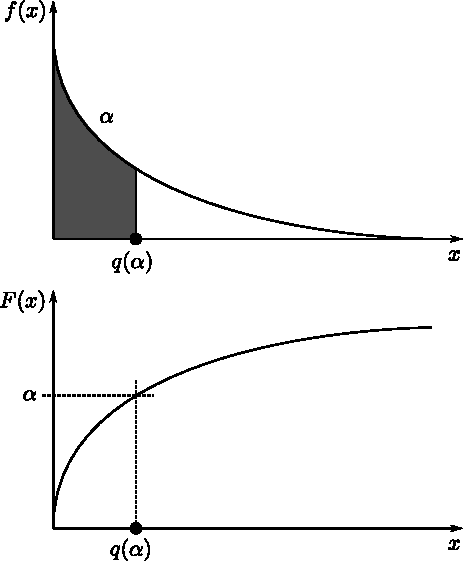
\includegraphics[scale=\graphscale]{dichtefunktion-quantile.pdf}
        \caption{Quantil $\alpha$ als Fläche in der Dichtefunktion $f(x)$ und
                 als Höhe in der kummulativen Verteilungsfunktion $F(x)$.}
\end{figure}


\subsection{Uniform}
\begin{Schunk}
\begin{Sinput}
> x=3;
> min=2;
> max=5;
> dunif(x=x,min=min,max=max)
\end{Sinput}
\begin{Soutput}
[1] 0.3333333
\end{Soutput}
\begin{Sinput}
> range=seq(from=0,to=10,by=0.001);
> plot(range,dunif(x=range,min=min,max=max),type='l')
\end{Sinput}
\end{Schunk}
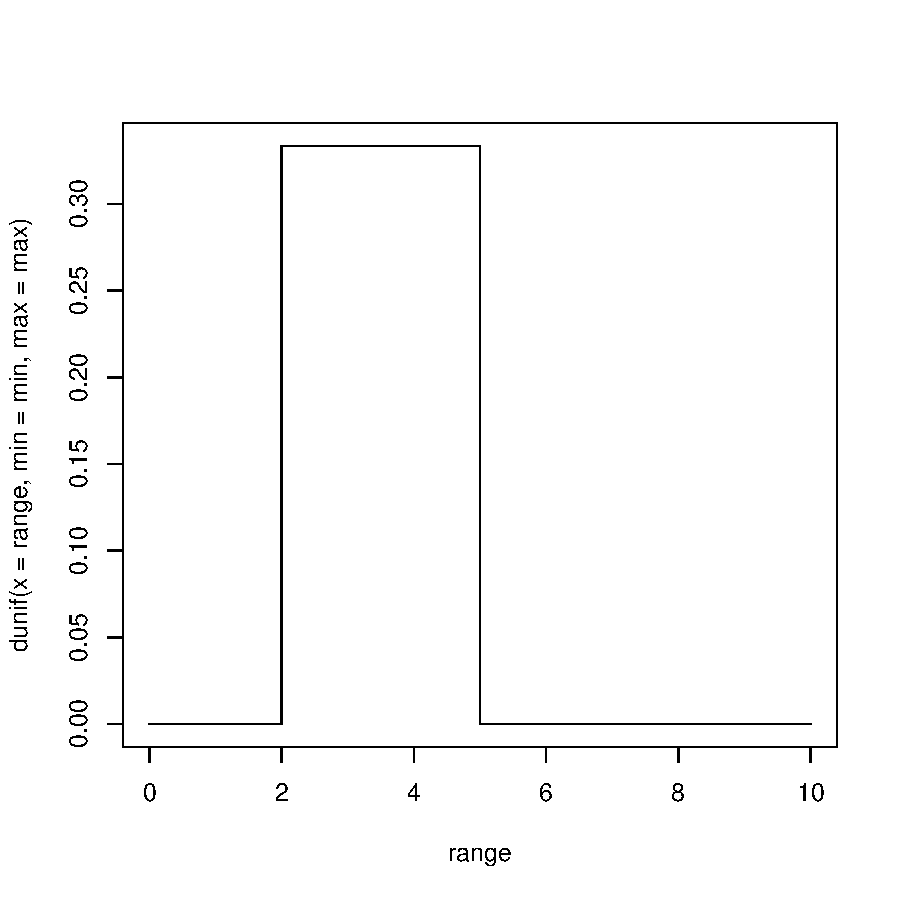
\includegraphics{definitionen-017}

\subsubsection{Erwartungswert}
\[ E(X) = \frac{\text{min} + \text{max}}{2} \]

\subsubsection{Varianz}
\[ Var(X) = \frac{(\text{max} - \text{min})^2}{12} \]

\subsubsection{Kumulative Verteilungsfunktion}
\begin{Schunk}
\begin{Sinput}
> q=3;
> punif(q=q,min=min,max=max)
\end{Sinput}
\begin{Soutput}
[1] 0.3333333
\end{Soutput}
\end{Schunk}

\subsection{Normalverteilung}
\begin{Schunk}
\begin{Sinput}
> x=7;
> mean=5;
> sd=1;
> dnorm(x=x,mean=mean,sd=sd)
\end{Sinput}
\begin{Soutput}
[1] 0.05399097
\end{Soutput}
\begin{Sinput}
> range=seq(from=0,to=10,by=0.001);
> plot(range,dnorm(x=range,mean=mean,sd=sd),type='l')
\end{Sinput}
\end{Schunk}
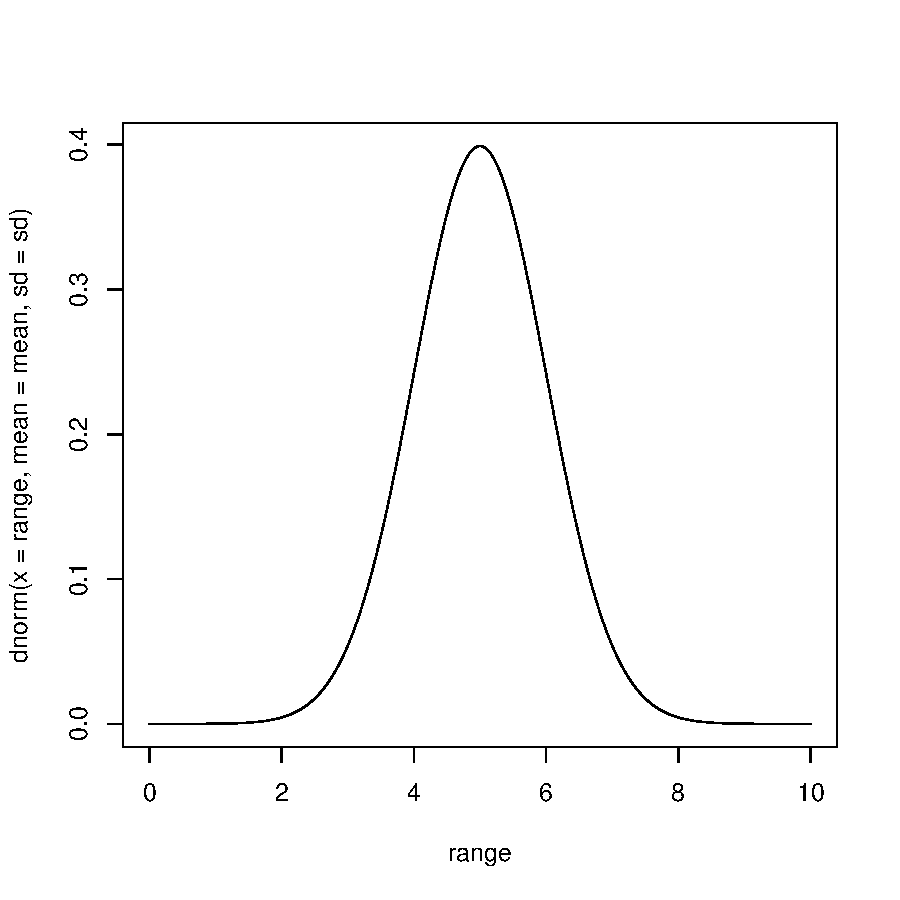
\includegraphics{definitionen-019}

\subsubsection{Erwartungswert}
\[ E(X) = \mu \]

\subsubsection{Varianz}
\[ Var(X) = \sigma^2 \]

\subsubsection{Kumulative Verteilungsfunktion}
\begin{Schunk}
\begin{Sinput}
> q=7;
> pnorm(q=q,mean=mean,sd=sd)
\end{Sinput}
\begin{Soutput}
[1] 0.9772499
\end{Soutput}
\end{Schunk}

\subsection{Exponentialverteilung}
\[ \begin{array}{@{}ll}
  \text{für }x \leq 0: & f(x) = \lambda \cdot e^{-\lambda \cdot x} \\
  \text{für }x < 0:    & f(x) = 0
\end{array} \]
\begin{Schunk}
\begin{Sinput}
> x=3;
> lambda=2;
> dexp(x=x,rate=lambda)
\end{Sinput}
\begin{Soutput}
[1] 0.004957504
\end{Soutput}
\begin{Sinput}
> range=seq(from=0,to=10,by=0.001);
> plot(range,dexp(x=range,rate=lambda),type='l')
\end{Sinput}
\end{Schunk}
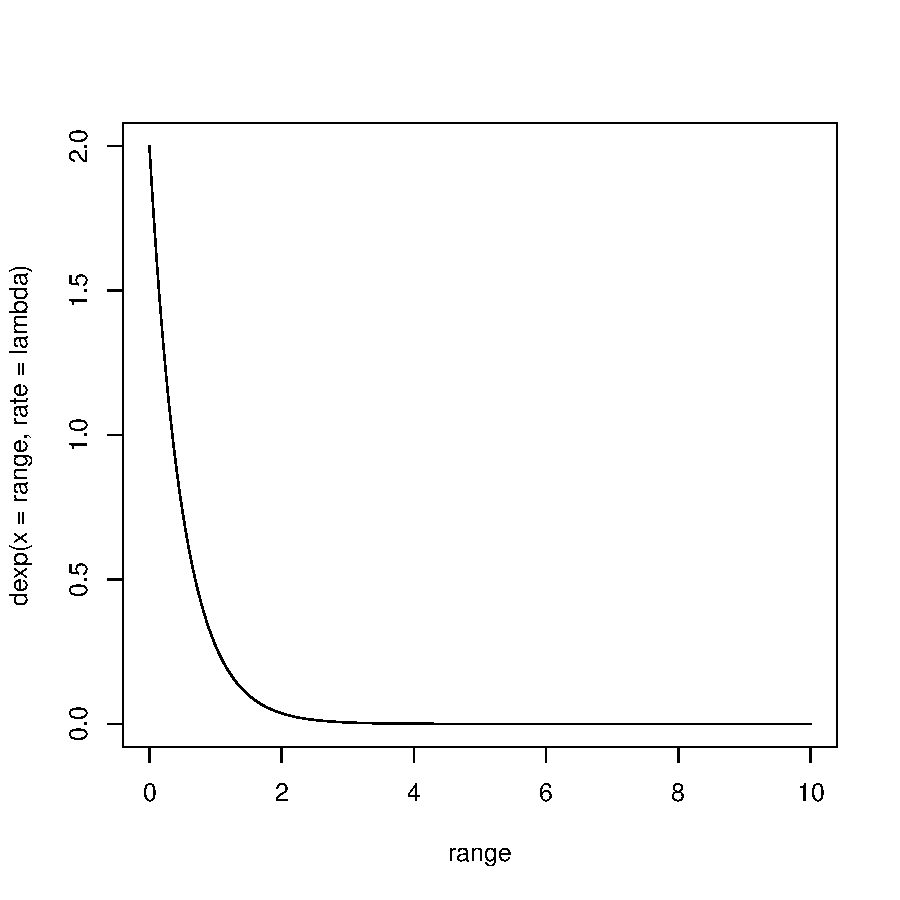
\includegraphics{definitionen-021}

\subsubsection{Erwartungswert}
\[ E(X) = \frac{1}{\lambda} \]

\subsubsection{Varianz}
\[ Var(X) = \frac{1}{\lambda^2} \]

\subsubsection{Kumulative Verteilungsfunktion}
\[ \begin{array}{@{}ll}
  \text{für }x \leq 0: & f(x) = 1 - e^{-\lambda \cdot x} \\
  \text{für }x < 0:    & f(x) = 0
\end{array} \]
\begin{Schunk}
\begin{Sinput}
> q=3;
> pexp(q=q,rate=lambda)
\end{Sinput}
\begin{Soutput}
[1] 0.9975212
\end{Soutput}
\end{Schunk}

\subsection{Übersicht Berechnung stetiger Verteilungen mit R}
\begin{tabular}{@{}lllll}
  \rowcolor{lgray}Verteilung &
    Dichte & 
    höchstens & 
    mindestens &
    Zufall \\
  Uniform &
    \verb!dunif(x=A,...)! &
    \verb!punif(q=A,...)! &
    \verb!1-punif(q=A,...)! &
    \verb!runif(n=...)!\\
  Normal &
    \verb!dnorm(x=A,...)! &
    \verb!pnorm(q=A,...)! &
    \verb!1-pnorm(q=A,...)! &
    \verb!rnorm(n=...)!\\
  Exponential &
    \verb!dexp(x=A,...)! &
    \verb!pexp(q=A,...)! &
    \verb!1-pexp(q=A,...)! &
    \verb!rexp(n=...)!\\
  t &
    \verb!dt(x=A,...)! &
    \verb!pt(q=A,...)! &
    \verb!1-pt(q=A,...)! &
    \verb!rt(n=...)!
\end{tabular}

\section{Statistischer Test}
Beim statistischen Test wird überprüft, ob eine statistische Verteilung zu 
ermittelten Daten passt. Dieser Test besteht aus 6 Schritten. 

\subsection{allgemeiner Ablauf}
\begin{enumerate}
  \item Modell \\
        Verteilung bestimmen
  \item Nullhypothese \\
        Nullhypothese und Alternativhypotese aufstellen
  \item Teststatistik \\
        Teststatistik aus Modell und Nullhypothese erstellen
  \item Signifikanzniveau \\
        Signifikanzniveau festlegen
  \item Verwerfungsbereich \\
        Aus Teststatistik und Signifikanzniveau Verwerfungsbereich berechnen
  \item Testentscheid \\
        Messwert mit Verwerfungsbereich vergleichen
\end{enumerate}

\subsection{Entscheidungsbaum}
\begin{figure}[h!]
  \centering
  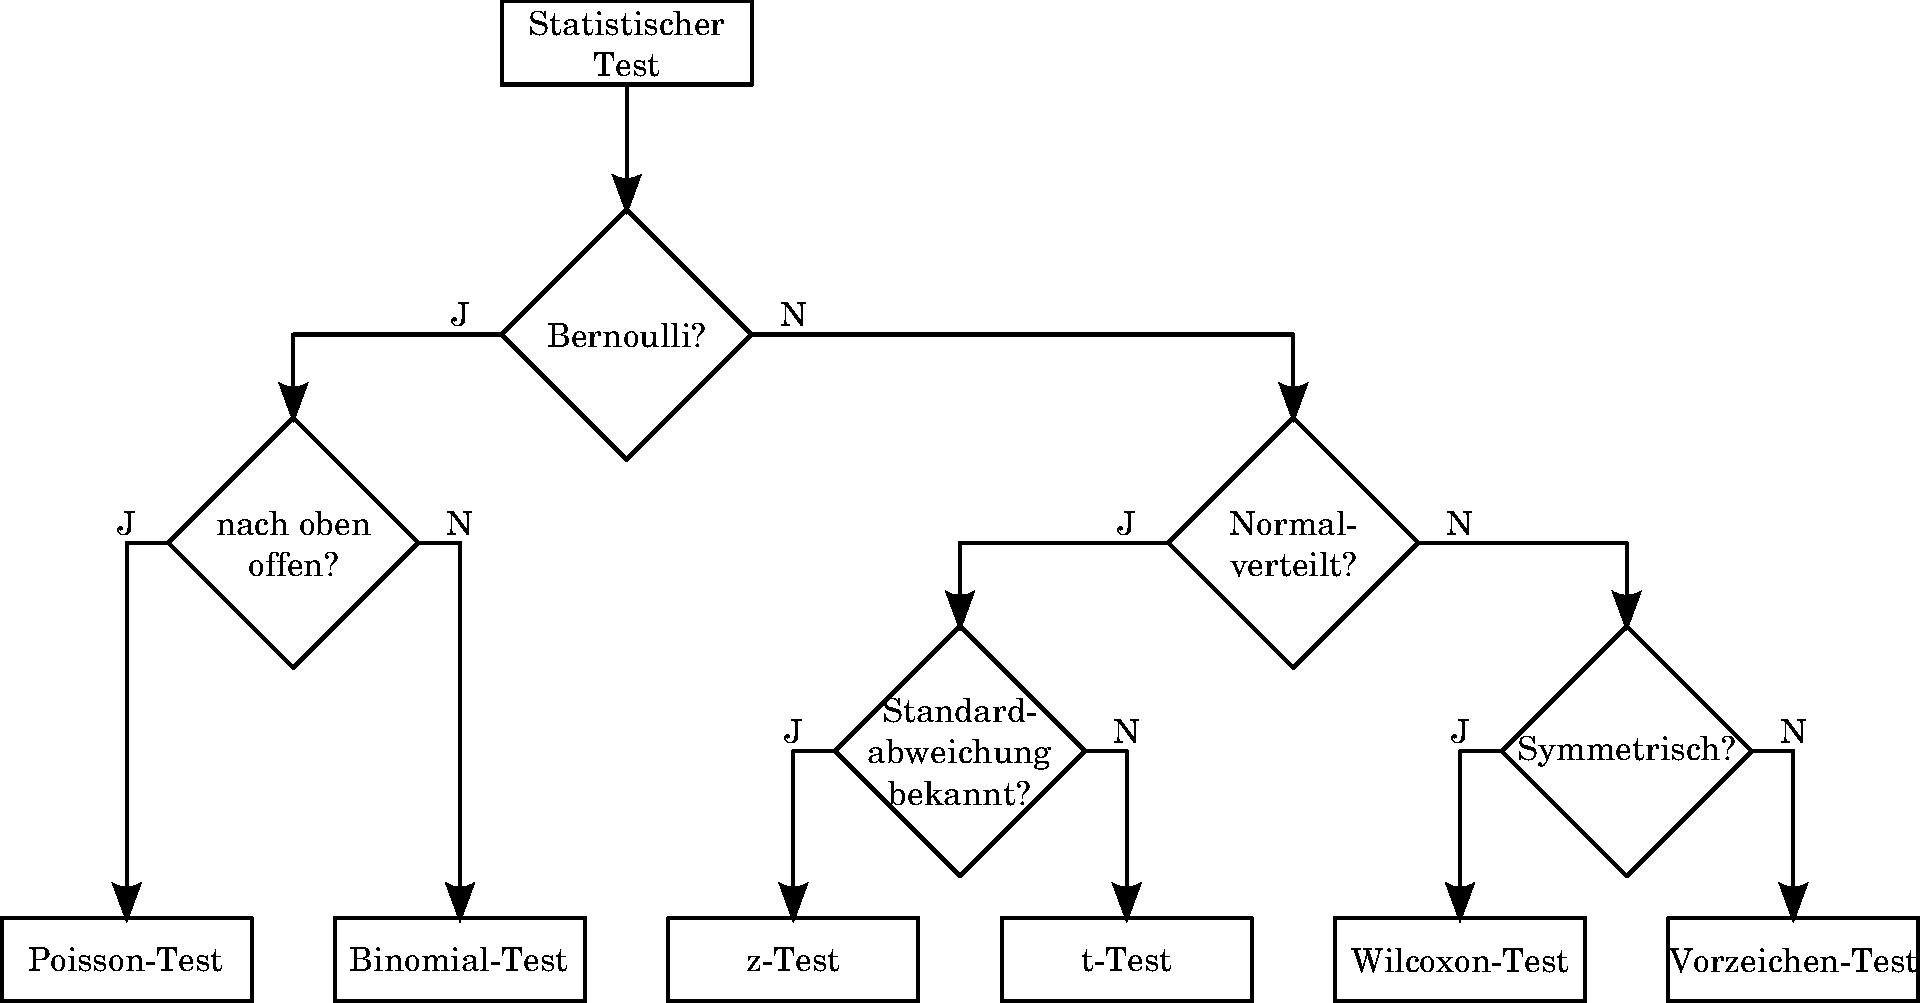
\includegraphics[width=1\textwidth]{testauswahl.pdf}
  \caption{Entscheidungsbaum für den statistischen Test}
\end{figure}

\subsection{Wirkungstabelle}
Ein Signifikanztest kann zu folgenden Entscheidungen führen.

\begin{table}[h!]
	\centering
	\begin{tabular}{l|lll}
	Entscheidung & Wirklichkeit: & & \\
	& $H_0$ ist wahr & $H_0$ ist falsch \\
	\hline
	&&& \\
	$H_0$ nicht verworfen & richtige Entscheidung & Fehler 2. Art \\
	&&& \\
	$H_0$ verworfen & Fehler 1. Art & richtige Entscheidung \\
	&&& \\
	\end{tabular}
\end{table}

\subsubsection{Fehler 1. Art}

\begin{figure}
        \centering
        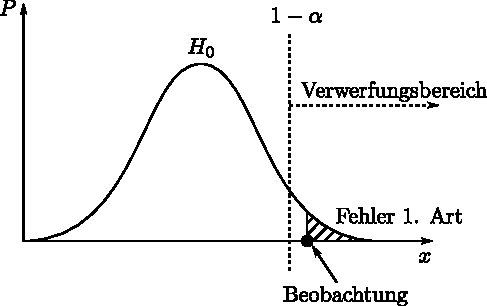
\includegraphics[scale=\graphscale]{fehler-erster-art.pdf}
        \caption{Fehler 1. Art}
\end{figure}

Der Fehler 1. Art tritt ein, wenn die Nullhypothese verworfen wird, 
obwohl sie wahr ist. Der Fehler 1. Art ist die Summe aller
Wahrscheinlichkeiten die extremer als die Beobachtung sind.
Der Fehler 1. Art kann also maximal so gross werden wie das
Signifikanzniveau $\alpha$, denn sonst wäre die Beobachtung ja
nicht im Verwerfungsbereich gewesen und die Hypothese nicht 
verworfen worden.

\subsubsection{Fehler 2. Art}
\begin{figure}
        \centering
        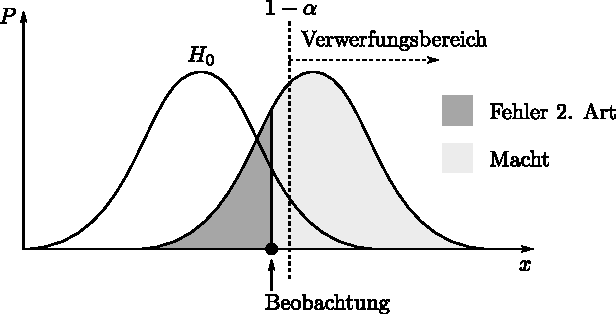
\includegraphics[scale=\graphscale]{fehler-zweiter-art.pdf}
        \caption{Fehler 2. Art}
\end{figure}

Der Fehler 2. Art tritt ein, wenn die Nullhypothese nicht verworfen
wird, obwohl die Alternative wahr ist. Wichtig ist hier zu verstehen,
dass dieser Fehler nur berechnet werden kann, wenn man eine alternative
Verteilung explizit bestimmt (denn man testet meist relativ d.h.
$p_A > p_0$, $p_A < p_0$ oder $p_A \neq p_0$).
Dabei gibt die sog. \emph{Macht} Auskunft darüber, wie Aussagekräftig
die annahme ist.
Der Fehler 2. Art ist die Summe aller Wahrscheinlichkeiten der alternativen
Verteilung, die weniger extrem als die Beobachtung sind.
Die Macht entspricht dann der Differenz von 1 zum Fehler 2. Art, 
d.h. Macht$=1-P(\text{Fehler 2. Art})$

\subsection{Binomial-Test}
Der Binomial-Test ist immer dann anzuwenden, wenn eine Binomialverteilung
vorliegt. Der Binomial-Test kann ein- oder zweiseitig erfolgen, d.h. das
Signifikanzniveau wird entweder von unten oder von oben angewendet (einseitig)
oder es wird geteilt auf den unteren und oberen Bereich (zweiseitig). 
Hierbei wird nicht zwingend symmetrisch geteilt, sondern nur dann wenn
die Verteilung symmetrisch ist.

% Hier das Beispiel mit den m&m's einfügen
\subsubsection*{Beispiel}
Wir haben eine Packung m\&m's gekauft und Jemand behauptet es habe
mehr gelbe m\&m's als in anderen Farben. Wir wollen das prüfen und
machen für jede Farbe einen statistischen Test.

\begin{enumerate}
	\item Modell: Binomial\\
	$X \sim Bin(n,p)$ mit $n=18$ (wir wissen es hat 18 m\&m's im Pack)\\
	$X \sim Bin(n=18, p)$
	\item Nullhypothese: $H_0$: $p_0 = \frac{1}{6}$ (es hat 6 Farben) \\
	Alternative: $H_A$: $p_A > p_0 = \frac{1}{6}$ 
	\item Teststatistik: \\
	$X$: $P(X=x|H_0)={n \choose x} p_0^x (1-p_0)^{n-x}$ \\
	$X$: $P(X=x|H_0)={18 \choose x} (\frac{1}{6})^x (1-\frac{1}{6})^{n-x}$
	\item Signifikanzniveau: $\alpha=0.05$
	\item Verwerfungsbereich:
	Wir ermitteln den Verwerfungsbereich mit Hilfe von R:
\begin{Schunk}
\begin{Sinput}
> round(1-pbinom(q=0:18, size=18, prob=1/6), 3)
\end{Sinput}
\begin{Soutput}
 [1] 0.962 0.827 0.597 0.352 0.168 0.065 0.021 0.005 0.001 0.000 0.000 0.000 0.000 0.000 0.000 0.000 0.000 0.000
[19] 0.000
\end{Soutput}
\end{Schunk}
	Vorsicht: Berechnet man den Verwerfungbereich mit R so muss man sehr
	darauf achten, was R einem liefert. Denn man kann sich hier leicht 
	irren lassen und sich um eine Stelle versetzt eindenken. Tipp: Denke
	daran, dass die Wahrscheinlichkeit, mindestens Null Treffer zu landen
	schon sprachlich absurd ist, also wird R auch bei 1 und nicht bei Null
	anfangen.\\
	Für uns ist der Verewerfungsbereich ab dem 7. Element (0.021) welches
	7 m\&m's entspricht (obwohl wir \verb!q=0:18! haben, steht das 1. Element
	für das 7. m\&m und nicht etwa das 6.).
	\item Testentscheid:\\
	
	\begin{table}[h!]
	\centering
	\begin{tabular}{c|c|c|c|c|c|c}
	Farbe & gelb & orange & rot & blau & grün & braun \\
	\hline
	gezählt & 3 & 1 & 6 & 4 & 1 & 3 \\
	\hline
	$H_0$ & behalten & behalten & behalten & behalten & behalten & behalten \\ 
	\end{tabular}
	\end{table}

	\noindent
	Keine der Farben liegt im Verwerfungsbereich, d.h. die Nullhypothese
	$H_0$ kann nicht verworfen werden.
\end{enumerate}


\subsection{z-Test}
Der z-Test ist ein Test für eine Normalverteilung $\mathcal{N}(\mu, \sigma^2)$


\begin{enumerate}
  \item Modell \\
	  $X_1,...,X_n$ \acs{i.i.d.} $\sim\mathcal{N}(\mu, \sigma_x^2)$ 
	wobei $\sigma_x$ bekannt ist
  \item Nullhypothese \\
       	$H_0$: $ \mu=\mu_0$ \\
	Alternativhypothese \\
	$H_A$: $ \mu \neq \mu_0 (\mu < \mu_0, \mu > \mu_0)$
  \item Teststatistik \\
	  $Z=\dfrac{\overline{X}_n-\mu_0}{\sigma_{\overline{X}_n}} = 
	  \dfrac{\sqrt{n}\cdot(\overline{X}_n-\mu_0)}{\sigma_x}
	  \qquad $ $\overline{X}_n$ ist der Mittelwert der Beobachtungen
	  \verb!mean()!\\
	  Verteilung der Teststatistik unter $H_0$\\
	  $Z\sim\mathcal{N}(0,1)\quad$ (sog. standardisierte Normalverteilung)
  \item Signifikanzniveau \\
        $\alpha= $\dots
  \item Verwerfungsbereich \\
	Hier ist wichtig zu beachten, dass es drei mögliche Formulierungen
	gibt:
	\begin{itemize}
		\item	Die Alternative kann beidseitig liegen \\
		$H_A$: $\mu\neq\mu_0 \Rightarrow 
	 	K=(-\infty, -\Phi^{-1}(1-\frac{\alpha}{2}]
		\cup [\Phi^{-1}(1-\frac{\alpha}{2}), \infty)$ \\
		\item Die Alternative wird linksseitig vermutet \\
		$H_A$: $\mu<\mu_0    \Rightarrow 
		K=(-\infty, -\Phi^{-1}(1-\alpha)] $ \\
		\item Die Alternative wird rechtsseitig vermutet \\
		$H_A$: $\mu>\mu_0    \Rightarrow 
		K=[\underbrace{\Phi^{-1}(1-\alpha)}_{\footnotesize
		\verb!qnorm(1-!\alpha\verb!,0,1)!}, \infty)$ \\
	\end{itemize}

  \item Testentscheid \\
	Wir prüfen ob $Z$ im Verwerfungsbereich $K$ liegt. Falls ja, 
	dann wird $H_0$ verworfen.
\end{enumerate}

\subsubsection{Beispiel mit R}
In R ist der z-Test nicht im Standardumfang dabei, da es ein Spezialfall 
des t-Test ist und nur zu Schulungszwecken verwendet werden sollte.
Man kann es aber manuell nachrüsten mit folgenden zwei Zeilen.\\
\begin{lstlisting}
install.packages('TeachingDemos')
library('TeachingDemos')
\end{lstlisting}

\noindent
Wir nehmen das Beispiel mit dem Weingeniesser, der prüfen möchte ob die 
Füllmengen richtig sind. Angeschrieben ist 70cl, desshalb ist unser
$\mu=70$. Die Standardabweichung ist 2. Beim z-Test kann man aber
auf drei mögliche Alternativen prüfen (beidseitig und je Seite einseitig), 
diese sind in R: \verb!less, greater, two.sided!. Im Fall des 
Weingeniessers müssen wir natürlich auf \verb!less! prüfen. 
Wir möchten das auf einem Signifikanzniveau von $\alpha=0.05$ testen.
\begin{Schunk}
\begin{Sinput}
> library('TeachingDemos')
> weinmenge <- c(71, 69, 67, 68, 73, 72, 71, 71, 68, 72, 69, 72)
> z.test(x=weinmenge, mu=70, sd=2, alternative='less')
\end{Sinput}
\begin{Soutput}
	One Sample z-test

data:  weinmenge 
z = 0.433, n = 12.000, Std. Dev. = 2.000, Std. Dev. of the sample mean = 0.577, p-value = 0.6675
alternative hypothesis: true mean is less than 70 
95 percent confidence interval:
     -Inf 71.19966 
sample estimates:
mean of weinmenge 
            70.25 
\end{Soutput}
\end{Schunk}

\noindent
Der P-Wert ist hier 0.6675, unser $\alpha$ ist aber 0.05, d.h. 
die Beobachtungen liegen nicht im Verwerfungsbereich!


\subsection{t-Test}
Der t-Test ist ein Test für eine Normalverteilung $\mathcal{N}(\mu, \sigma^2)$, 
wenn $\sigma_x$ nicht bekannt ist. $\hat{\sigma}_x$ wird dann aus den Messdaten 
geschätzt. Mit R geschieht das mit dem Befehl \verb!sd()!. Dadurch ändert sich 
die Teststatistik zu einer t-Verteilung. 

\begin{enumerate}
  \item Modell \\
	  $X_1,...,X_n$ \acs{i.i.d.} $\sim\mathcal{N}(\mu, \sigma_x^2)$ 
	wobei $\sigma_x$ durch $\hat{\sigma}_x$ geschätzt wird
  \item Nullhypothese \\
       	$H_0$: $ \mu=\mu_0$ \\
	Alternativhypothese \\
	$H_A$: $ \mu \neq \mu_0 (\mu < \mu_0, \mu > \mu_0)$
  \item Teststatistik \\
	  $T=\dfrac{\sqrt{n}\cdot(\overline{X}_n-\mu_0)}{\hat{\sigma}_x}
      \qquad $ $\overline{X}_n$ ist der Mittelwert der Beobachtungen
	  \verb!mean()!\\
	  Verteilung der Teststatistik unter $H_0$\\
	  $T \sim t_{n-1}$
  \item Signifikanzniveau \\
        $\alpha= $\dots
  \item Verwerfungsbereich \\
	Hier ist wichtig zu beachten, dass es drei mögliche Formulierungen
	gibt:
	\begin{itemize}
		\item	Die Alternative kann beidseitig liegen \\
		$H_A$: $\mu\neq\mu_0 \Rightarrow 
	 	K=(-\infty, -t_{n-1;1-\frac{\alpha}{2}}]
		\cup [t_{n-1;1-\frac{\alpha}{2}}, \infty)$ \\
		\item Die Alternative wird linksseitig vermutet \\
		$H_A$: $\mu<\mu_0    \Rightarrow 
		K=(-\infty, -t_{n-1;1-\alpha}] $ \\
		\item Die Alternative wird rechtsseitig vermutet \\
		$H_A$: $\mu>\mu_0    \Rightarrow 
		K=[t_{n-1;1-\alpha}, \infty)$ \\
	\end{itemize}
    $t_{n-1;1-\alpha}$ muss dabei aus einer Tabelle entnommen oder mit R 
    berechnet werden. \\
    \verb!qt(p=!$\alpha$\verb!,df=!$n$\verb!)!
  \item Testentscheid \\
	Wir prüfen ob $T$ im Verwerfungsbereich $K$ liegt. Falls ja, 
	dann wird $H_0$ verworfen.
\end{enumerate}

\subsubsection{Beispiel mit R}
Wir nehmen erneut das Beispiel mit dem Weingeniesser, der prüfen möchte ob die 
Füllmengen richtig sind. Angeschrieben ist 70cl, deshalb ist unser $\mu=70$. 
Die Standardabweichung wird nun aber durch R aus den Messungen geschätzt. 
Beim t-Test kann man auch auf drei mögliche Alternativen prüfen 
(beidseitig und je Seite einseitig), diese sind in R: 
\verb!less, greater, two.sided!. Im Fall des Weingeniessers müssen wir 
natürlich auf \verb!less! prüfen. Wir möchten das auf einem Signifikanzniveau 
von $\alpha=0.05$ testen.
\begin{Schunk}
\begin{Sinput}
> weinmenge <- c(71, 69, 67, 68, 73, 72, 71, 71, 68, 72, 69, 72)
> t.test(x=weinmenge, mu=70, alternative='less')
\end{Sinput}
\begin{Soutput}
	One Sample t-test

data:  weinmenge 
t = 0.4419, df = 11, p-value = 0.6664
alternative hypothesis: true mean is less than 70 
95 percent confidence interval:
     -Inf 71.26603 
sample estimates:
mean of x 
    70.25 
\end{Soutput}
\end{Schunk}

\noindent
Der P-Wert ist hier 0.6664, unser $\alpha$ ist aber 0.05, d.h. 
die Beobachtungen liegen nicht im Verwerfungsbereich!


\subsection{Wilcoxon Rangsummen Test}
Der Wilcoxon Rangsummen Test wird auf Verteilungen angewendet, die keine 
Normalverteilung aufweisen und symmetrisch verteilt sind. Im Rahmen des Moduls 
Stochastik wird nicht auf die Berechnung des Wilcoxon Rangsummen Tests 
eingegangen. Berechnung in R: 
\begin{Schunk}
\begin{Sinput}
> wilcox.test(x=weinmenge,mu=70,alternative='less')
\end{Sinput}
\begin{Soutput}
	Wilcoxon signed rank test with continuity correction

data:  weinmenge 
V = 44.5, p-value = 0.6838
alternative hypothesis: true location is less than 70 
\end{Soutput}
\end{Schunk}

\subsection{Vorzeichen-Test}
Beim Vorzeichentest werden die Daten mit dem Median verglichen. Dieser Median 
darf aber nicht aus den Daten gebildet werden, sondern muss bekannt sein 
(z.B. aus der Nullhypothese ($\mu_0$)). Ist ein Datenpunkt grösser als der 
Median wird er als positiv betrachtet, ansonsten als negativ. Darauf kann dann 
ein Binomialtest angewendet werden. 
\subsubsection{Vorzeichentest mit R}
Für den Vorzeichentest muss zunächst jeder Datenpunkt mit dem Median verglichen 
werden. Das kann man in R mit \verb!>! gemacht werden. \\
% \verb!binom.test(x=sum(data>mu),length(data),p=0.5,alternative='less',conf.level=0.95)!
\begin{Schunk}
\begin{Sinput}
> data=runif(120,10,35)               # Daten erfassen
> mu=25                               # Median erfassen
> # Vorzeichentest
> binom.test(x=sum(data>mu),length(data),p=0.5,alternative='less',conf.level=0.95)
\end{Sinput}
\begin{Soutput}
	Exact binomial test

data:  sum(data > mu) and length(data) 
number of successes = 52, number of trials = 120, p-value = 0.08532
alternative hypothesis: true probability of success is less than 0.5 
95 percent confidence interval:
 0.0000000 0.5125242 
sample estimates:
probability of success 
             0.4333333 
\end{Soutput}
\end{Schunk}

\subsection{gepaarter Test}
Bei einem Test mit zwei Messreihen mit jeweils den identischen Bedingungen, 
(z.B. beide Tests mit dem gleichen Individuum) kann ein gepaarter Test 
durchgeführt werden. Dafür wird für jeden Messpunkt die Differenz der 
Datenreihen verwendet und mit dieser neuen Datenreihe weitergerechnet. 

\subsubsection{gepaarter Test mit R}
Für einen gepaarten Test muss die Option \verb!paired=TRUE! verwendet werden. \\
\verb!t.test(x=data1,y=data2,alternative='less',paired=TRUE)!

\subsection{ungepaarter Test}
Der ungepaarte Test muss für das Modul STOC nur mit R berechnet werden. 

\subsubsection{ungepaarter Test mit R}
Dafür kann die Option \verb!paired=FALSE! verwendet werden. Diese ist per 
Default so gesetzt, wenn der Test mit zwei Datenreihen durchgeführt wird. \\
\verb!t.test(x=man,y=fem,alternative='less',paired=FALSE)!\\

\subsubsection{gleiche Varianz}
Besitzen die beiden Datenreihen die gleiche Varianz, so muss das mit der Option 
\verb!var.equal=TRUE! definiert werden. \\
\verb!t.test(x=data1,y=data2,alternative='less',paired=FALSE,var.equal=TRUE)!

\section{P-Wert}
Der P-Wert (engl. oder R \emph{P-Value}) ist die Summe der 
Wahrscheinlichkeiten, welche die Beobachtung
und alle extremeren Beobachtungen vereint. Im folgenden Beispiel wärde dies
die Summe aller Wahrscheinlichkeiten rechts von der Beobachtung (20).

\begin{Schunk}
\begin{Sinput}
> plot(dbinom(x=0:30, size=30, prob=0.5), type='h')
> abline(v=20, col='red')
\end{Sinput}
\end{Schunk}
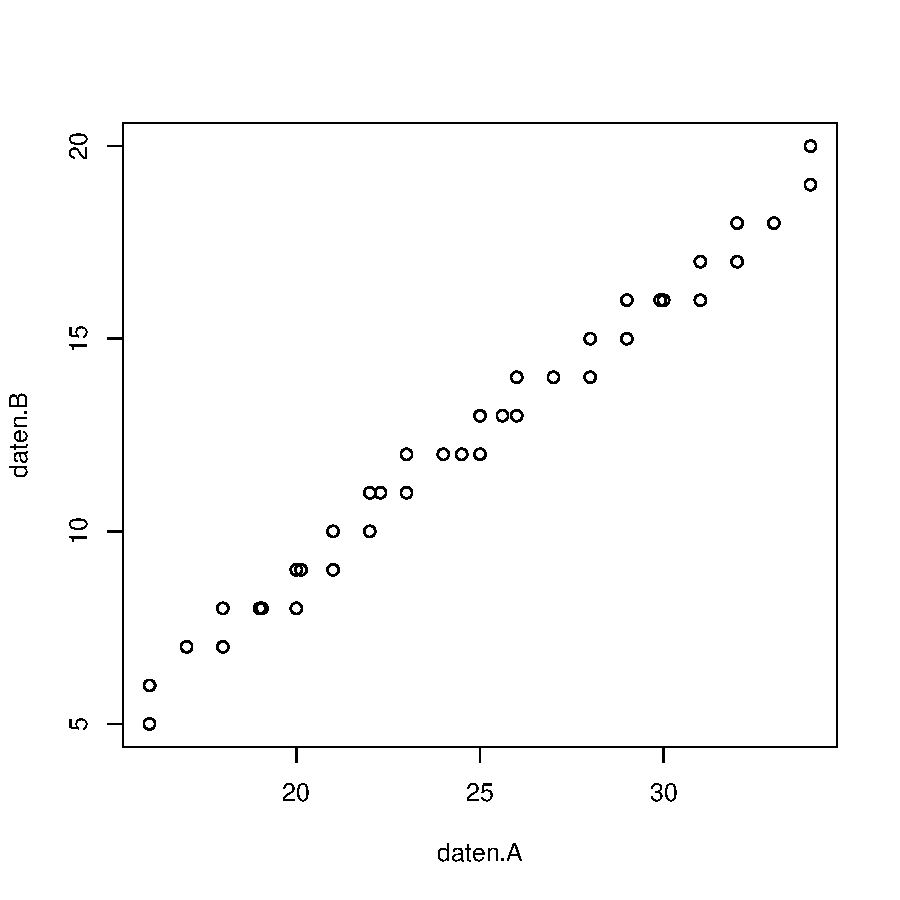
\includegraphics{definitionen-028}

\noindent
Der P-Value wird also genau gleich wie das $\alpha$-Quantil berechnet.
Für statistische Tests können wir mit Hilfe des P-Wertes das Berechnen
des Verwerfungsbereiches auslassen indem wir den P-Wert und unser
Signifikanzniveau vergleichen. Ist der P-Wert kleiner als das 
Signifikanzniveau, so liegt die Beobachtung im Verwerfungsbereich
und umgekehrt.

\section{QQ-Plot}
Wir wollen wissen ob zwei Datensätze (Verteilungen) von selben Typ sind.
Hierzu kann der sog. QQ-Plot gemacht werden. Sind die beiden Datensätze
vom selben Typ, d.h. ähnlich verteilt, so erhält man eine Gerade im 
QQ-Plot. Sind die Verteilungen nicht gleich, so gibt es keine Gerade. 

\begin{Schunk}
\begin{Sinput}
> daten.A <- rbinom(n=500, size=50, prob=0.5)
> daten.B <- rbinom(n=250, size=25, prob=0.5)
> # zwei Datensätze mit gleichem Typ der Verteilung
> qqplot(daten.A, daten.B)
\end{Sinput}
\end{Schunk}
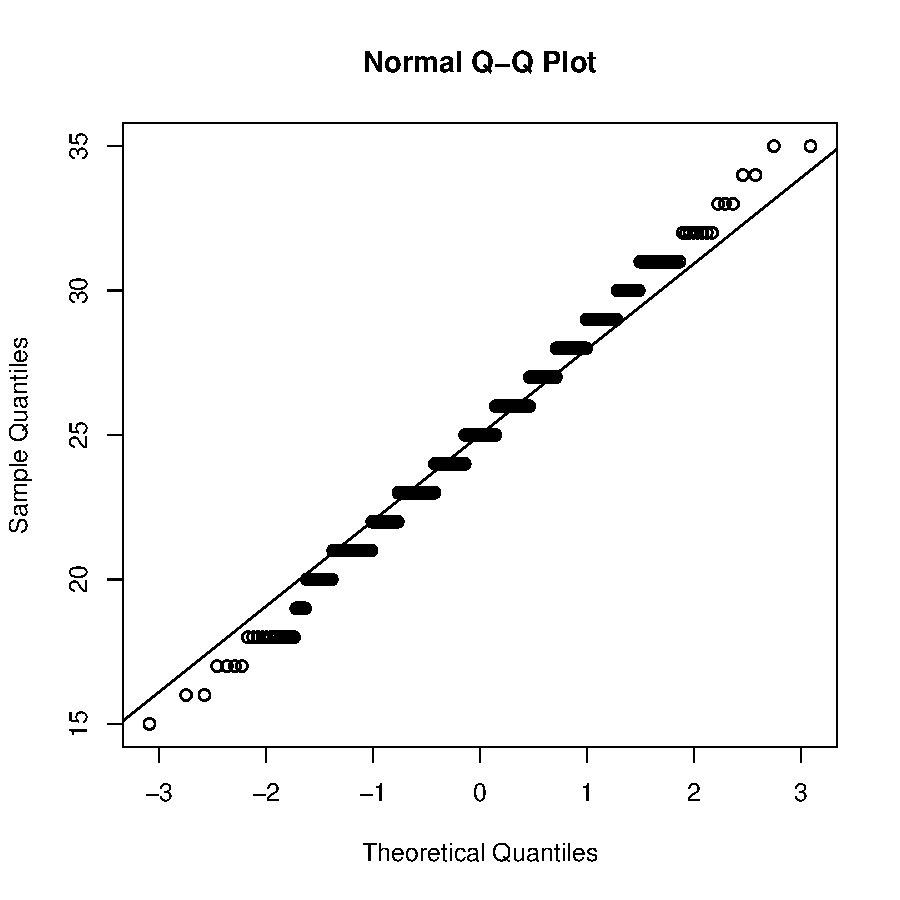
\includegraphics{definitionen-029}

\subsection{QQ-Norm}
Oft hat man aber nur eine Datenreihe die man auf eine bestimmte 
Verteilung testen möchte. Die wichtigste Verteilung ist die
Normalverteilung, daher gibt es eine spezielle R-Funktion um
eine Datenreihe gegen die Normalverteilung zu vergleichen.

\begin{Schunk}
\begin{Sinput}
> daten.A <- rbinom(n=500, size=50, prob=0.5)
> qqnorm(daten.A)
> # reale Linie ziehen 
> qqline(daten.A)
\end{Sinput}
\end{Schunk}
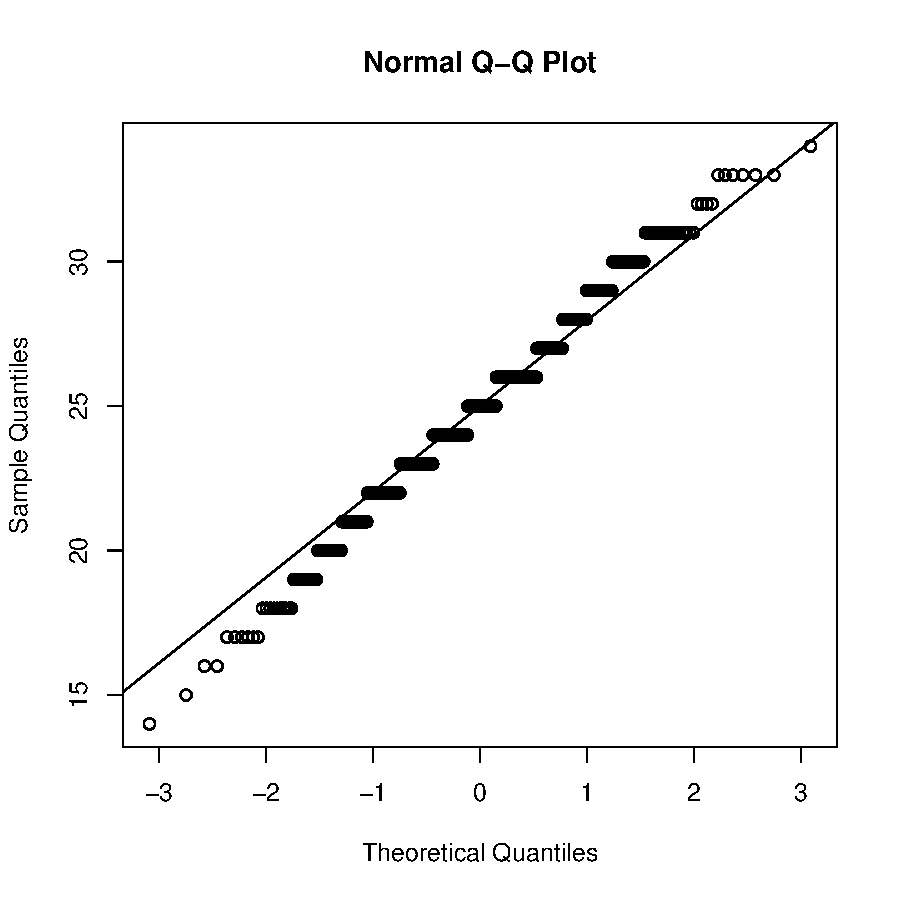
\includegraphics{definitionen-030}

\noindent
Im Beispiel wird eine Datenreihe welche binomialverteilt ist gegen
die Normalverteilung verglichen. Dabei stimmt es zwar soweit, dass
es eine Gerade gibt, nur sind darin Unterbrüche. Diese kommen daher, 
dass die Binomialverteilung diskret ist (d.h. nur ganzzahlig) und
die Normalverteilung stetig. Man kann aber verschiedene diskrete
Verteilungen voneinander unterscheiden in der \verb!qqnorm()!-Ausgabe.
Eine Poissonverteilung hat eine andere Charakterisitik als eine
Binomialverteilung.

\begin{Schunk}
\begin{Sinput}
> # ideal normalverteilte Datenreihe (mit Randomfunktion generiert)
> daten.ideal <- rnorm(n=1000, mean=5, sd=1)
> # reale poissonverteilte Datenreihe (mit Randomfunktion generiert)
> daten.C <- rpois(n=1000, lambda=5)
> qqnorm(daten.C)
> qqline(daten.ideal)
> qqline(daten.C)
\end{Sinput}
\end{Schunk}
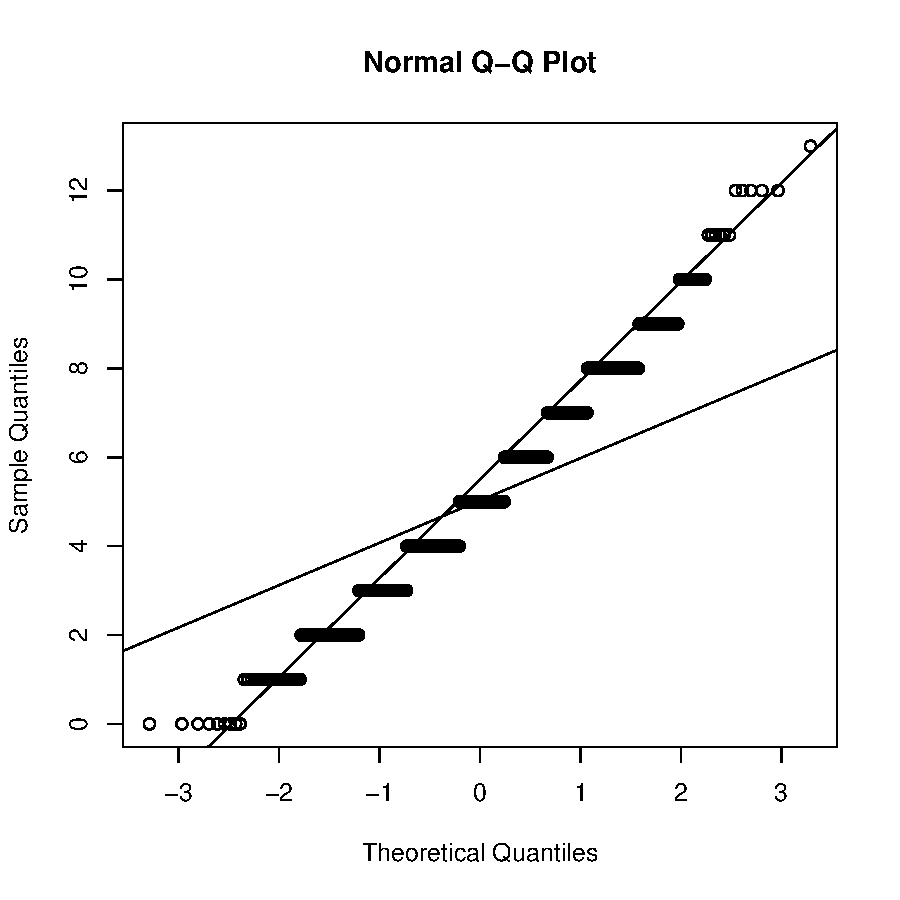
\includegraphics{definitionen-031}

\noindent
Im Beispiel ist deutlich zu sehen, dass die ideale und die reale Line 
sich nicht überlappen. D.h. die Daten haben nicht die selbe Verteilung
bzw. die Datenreihe ist nicht normalverteilt.

\subsubsection{Charakteistische Kurvenformen}

\begin{figure}[h!]
        \centering
        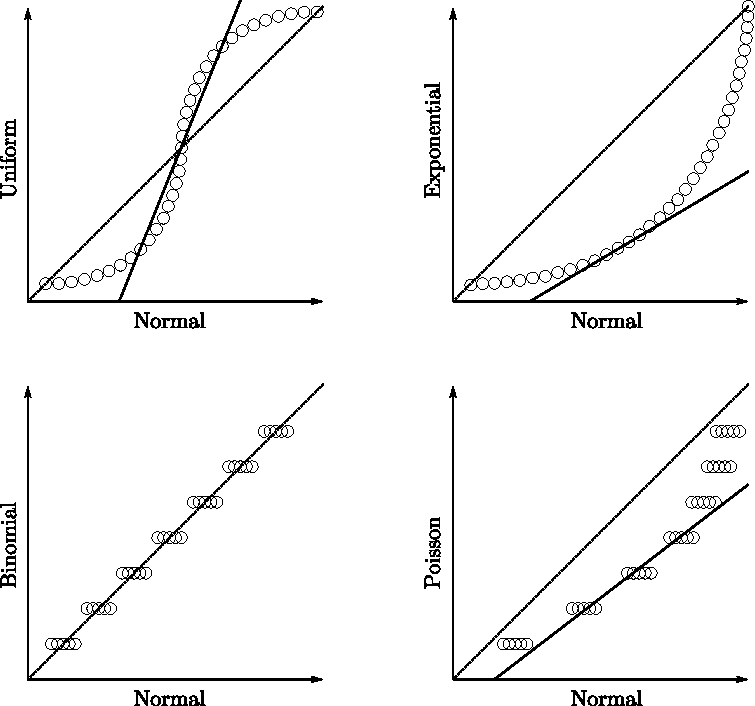
\includegraphics[scale=\graphscale]{qqnorm-kurven.pdf}
        \caption{Vergleich charakteristischer Verteilungen im qqnorm-Plot}
\end{figure}

\section{Regression}

\subsection{Definition}
\[ Y = \beta_0 + \beta_1 \cdot x + \epsilon \]

\subsubsection{Linear}
Kommt der Parameter $\beta_1$ nur in der ersten Potenz vor, so nennt man die
Regression linear.

\subsubsection{Einfach}
Kommt die unabhängige Variable $x$ nur in der erten Potenz vor, so nennt man 
die Regression einfach.

\subsubsection{Residuen}
\emph{Residuum} ist ein anderes Wort für Rest (Abweichung, Fehler),
\emph{Residuen} ist das Plural davon.
Spricht man bei der Regression von einem Residuum, so meint man damit z.B.
die Abweichung von den Daten zu dem Idealwerten die man erhält (bei Anwendung
der ermittelten Parameter $\beta_0$ und $\beta_1$).

\subsubsection{lm(\ldots)}
Mit \verb!lm()! kann die lineare Regression in R durchgeführt  werden. Dabei 
muss als erste Variable die y-Achse gefolgt von $\sim$ und der x-Achse angegeben 
werden. \\
\verb!lm(y !$\sim$\verb! x)!

\subsubsection{summary(lm(\dots))}
\verb!lm()! ermittelt die Parameter für die einfache lineare Regression, d.h.
es ermittelt $\beta_0$ und $\beta_1$.
\verb!summary(lm())! zeigt alle relevanten Daten der Regression an.
\begin{table}[h!]
	\centering
	\begin{tabular}{l|l|l}
	Parameter & Wo im \verb!lm()! & Beschreibung\\
	\hline
	$\beta_0$ & Coefficients: (Intercept) & Verschiebung in y-Richtung \\
	$\beta_1$ & Coefficients: 'daten' & Steigung \\
	\end{tabular}
	\caption{Daten die man aus dem lm() erhält}
\end{table}

\begin{table}[h!]
	\centering
	\begin{tabular}{l|l|p{0.4\textwidth}}
	Parameter & Wo im \verb!summary(lm())! & Beschreibung\\
	\hline
	$\beta_0$ & Estimate (Intercept) & Verschiebung in y-Richtung \\
	$\beta_1$ & Estimate 'daten' & Steigung \\
	$s.e.(\beta_0)$ & Std. Error (Intercept) & Standardabweichung der Verschiebung in y-Richtung\\
	$s.e.(\beta_1)$ & Std. Error (Intercept) & Standardabweichung der Steigung\\
	P-Wert für $\beta_0$ & Pr(>|t|) (Intercept) & Wahrscheinlichkeit, dass Verschiebung in y-Richtung 0 ist \\
	P-wert für $\beta_1$ & Pr(>|t|) & Wahrscheinlichkeit, dass die Steigung 0 ist\\
	$\varepsilon_1$ & Residual standard error & Rauschen um die Steigung und Verschiebung zu y\\
	$n-p$ & degrees of freedom & Freiheitsgrade ($n$ Beobachtungen - $p$ Parameter)\\
	\end{tabular}
	\caption{Daten die man aus dem summary(lm()) erhält}
\end{table}


\subsubsection{fitted() und resid()}



\subsection{Vertrauensintervall}
Das Vertrauensintervall gibt an, wie verlässlich die berechneten Parameter
sind für $\beta_0$ (y-Achsenabschnitt für x=0) und $\beta_1$ (die Steigung).
\subsubsection{Berechnung für $\beta_0$}
\[ \text{Untere Grenze} = \beta_0 - s.e.(\beta_0)\cdot t_{n-2;1-\frac{\alpha}{2}} \]
\[ \text{Obere Grenze} = \beta_0 + s.e.(\beta_0)\cdot t_{n-2;1-\frac{\alpha}{2}} \]
Dies kann man aus dem \verb!summary(lm(...))! berechnen mit den folgendne Daten:\\
\verb!Estimate (Intercept) !$\pm$\verb! Std.Error (Intercept)*qt(1-(alpha/2), df = Degree of Freedom)!
\subsubsection{Berechnung für $\beta_1$}
\[ \text{Untere Grenze} = \beta_1 - s.e.(\beta_1)\cdot t_{n-2;1-\frac{\alpha}{2}} \]
\[ \text{Obere Grenze} = \beta_1 + s.e.(\beta_1)\cdot t_{n-2;1-\frac{\alpha}{2}} \]
Wie beim $\beta_0$ können auch hier alle Daten aus dem 
\verb!summary(lm(...))! entnommen werden\\
\verb!Estimate 'daten' !$\pm$\verb! Std.Error 'daten'*qt(1-(alpha/2), df = Degree of Freedom)!



\section{Abkürzungsverzeichnis}
\begin{acronym}[SQL]
	\acro{i.i.d.}{Identically Identipednent Distributed}
\end{acronym}


